\subsection{Bedienung des Editors}
Der Editor ist über den Text-, Draw-, Shape- oder Image-Button erreichbar. Inital wird ein Choose file-Button abgebildet. Je nachdem, ob nach erstmaligem Öffnen einer PDF-Datei auf Text, Draw, Shape oder Image geklickt wurde, wird als erstes der Writer-, Drawer-, Shaper- oder Imager-Bearbeitungsmodus zugänglich gemacht. Ist eine Datei geöffnet, so ist der Reader ohne die Operationen zum Seiten Drehen Teil jedes Editormoduls. Alle input fields im Editor sind mit dem gültigen Wertebereich für Benutzereingaben als Information Min: Max: versehen. Der Editor samt gerendertem Dokument besteht aus einem grauen, waagerechten Operations Bar, einem linken Layers Seitenmenü in Rosa und einem rechten grünen Tools Seitenmenü. Mit dem linken, äußeren, grünen Button Layers im Operations Bar kann das Layers Seitenmenü aus- bzw. eingeblendet werden. Der benachbarte Button Tools zeigt bzw. verbirgt das Tools Seitenmenü. Standardmäßig sind Layers und Tools ausgeklappt. Nach Dateiauswahl informiert eine Infobox über den Renderfortschritt der Seiten. Ebenso gibt eine Infobox Auskunft über den Speicherprozess. Wurden Text, Drawings, Shapes oder Images hinzugefügt und Save betätigt, zoomt das Dokument zunächst auf 500 \%, damit die Elemente als PNG-Bilder in hochwertiger Qualität eingebettet werden können. Am Ende des Speichervorgangs wird der vorherige Zoomwert wiederhergestellt. Beide Infoboxen, die in Screenshot \ref{fig:render-info} und \ref{fig:save-info} abgebildet sind, werden auch im Reader eingeblendet. Die einzelnen Speicherschritte werden in der Webkonsole der Web Developer Tools des Browsers ausgegeben, was in Bild \ref{fig:save-progress-steps} zu sehen ist.

\begin{figure}[!htbp]
	\centering
	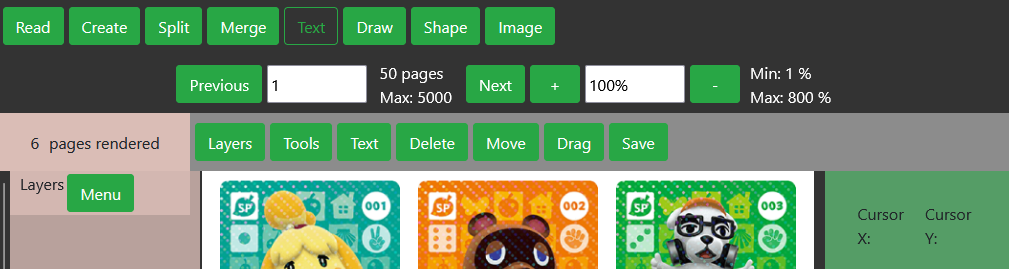
\includegraphics[width=1\textwidth]{"images/render-info.png"}
	\caption{Infobox über den Renderfortschritt der PDF Web App}
	\label{fig:render-info}
\end{figure}

\begin{figure}[!htbp]
	\centering
	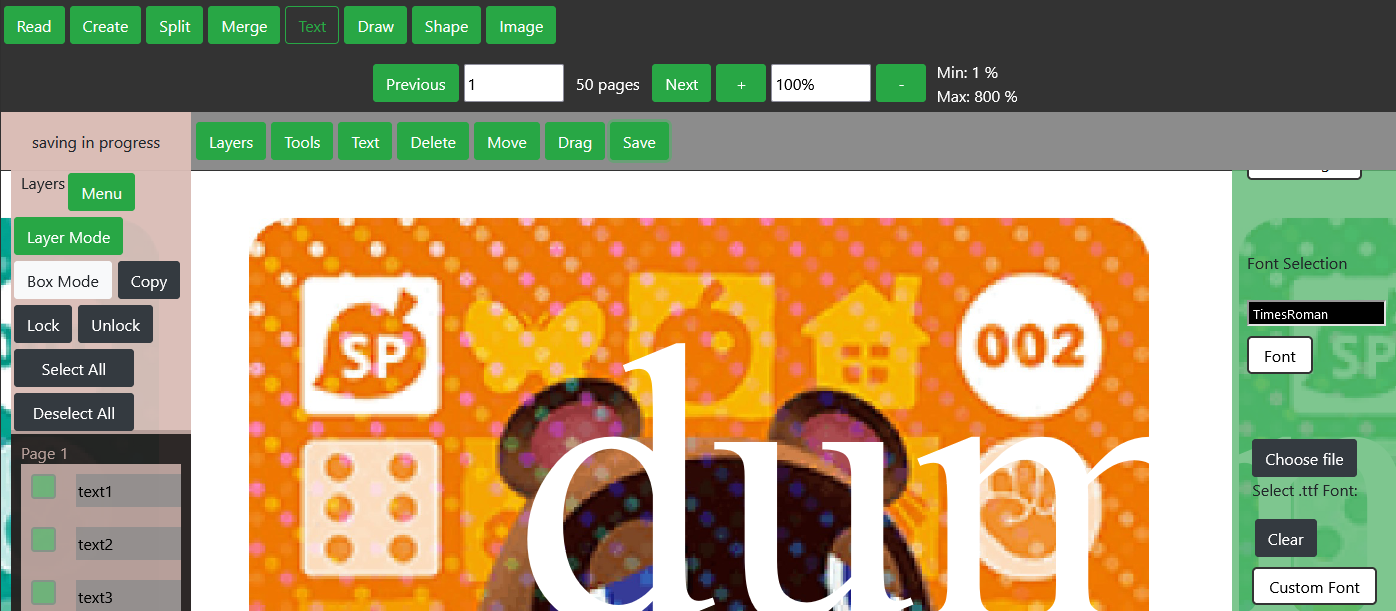
\includegraphics[width=1\textwidth]{"images/save-info.png"}
	\caption{Infobox über den Speicherprozess der PDF Web App}
	\label{fig:save-info}
\end{figure}

\begin{figure}[!htbp]
	\centering
	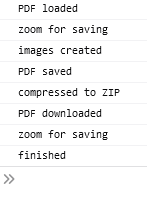
\includegraphics[width=0.4\textwidth]{"images/save-progress-steps.png"}
	\caption{Speicherschritte der PDF Web App in der Webkonsole beim Speichern von Elementen}
	\label{fig:save-progress-steps}
\end{figure}

\subsubsection{Textbearbeitung}
Wurde der Writer aufgerufen, präsentiert sich er Texteditor in den Abbildungen \ref{fig:texteditor} und \ref{fig:texteditor2}.

\begin{figure}[!htbp]
	\centering
	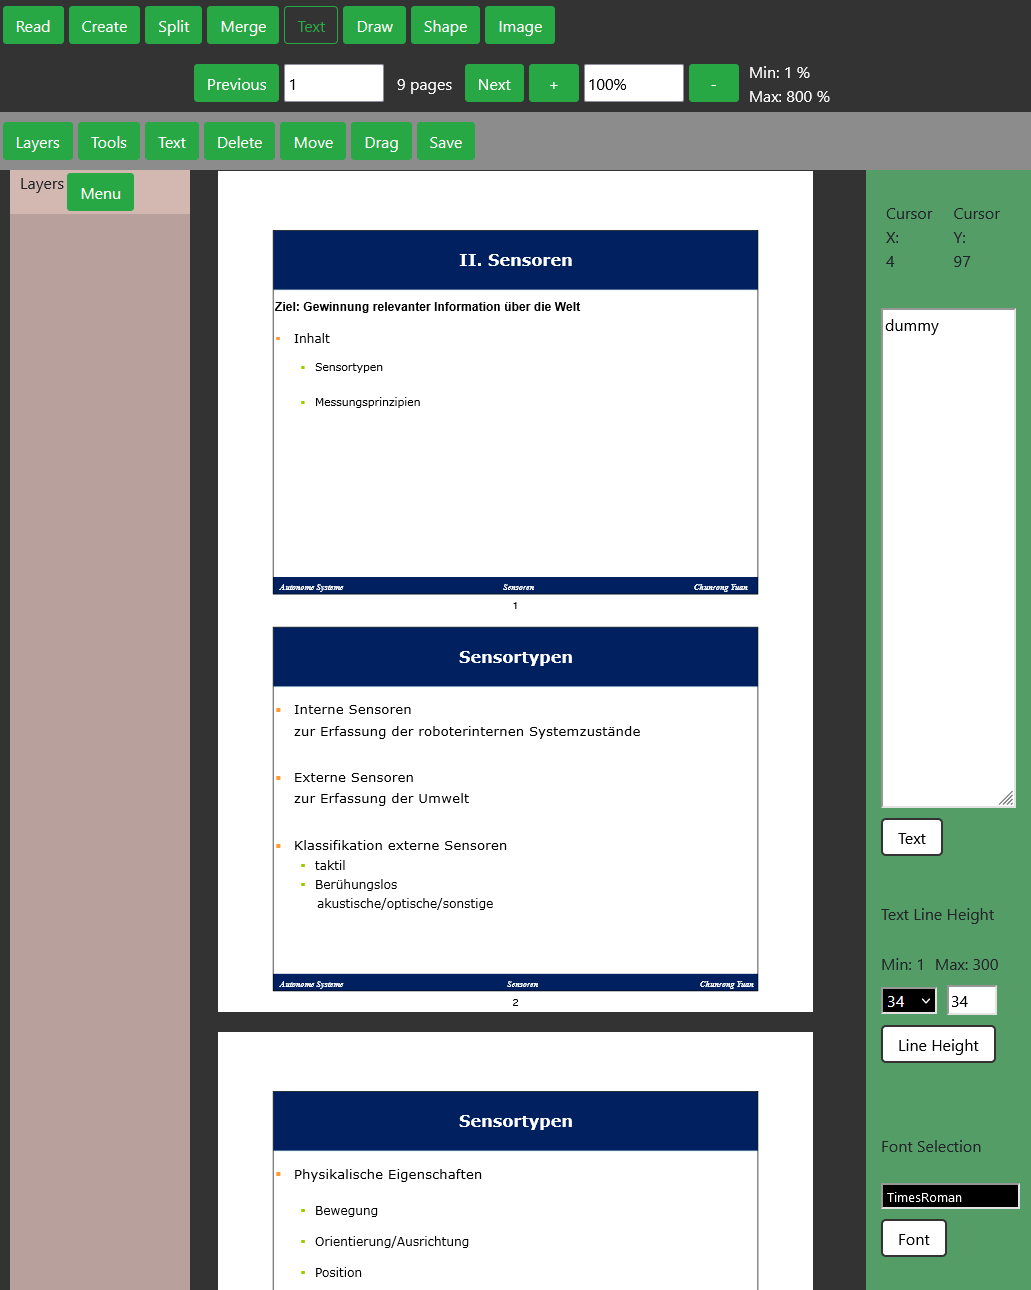
\includegraphics[width=1\textwidth]{"images/texteditor.png"}
	\caption{Startseite des Writers der PDF Web App}
	\label{fig:texteditor}
\end{figure}

\begin{figure}[!htbp]
	\centering
	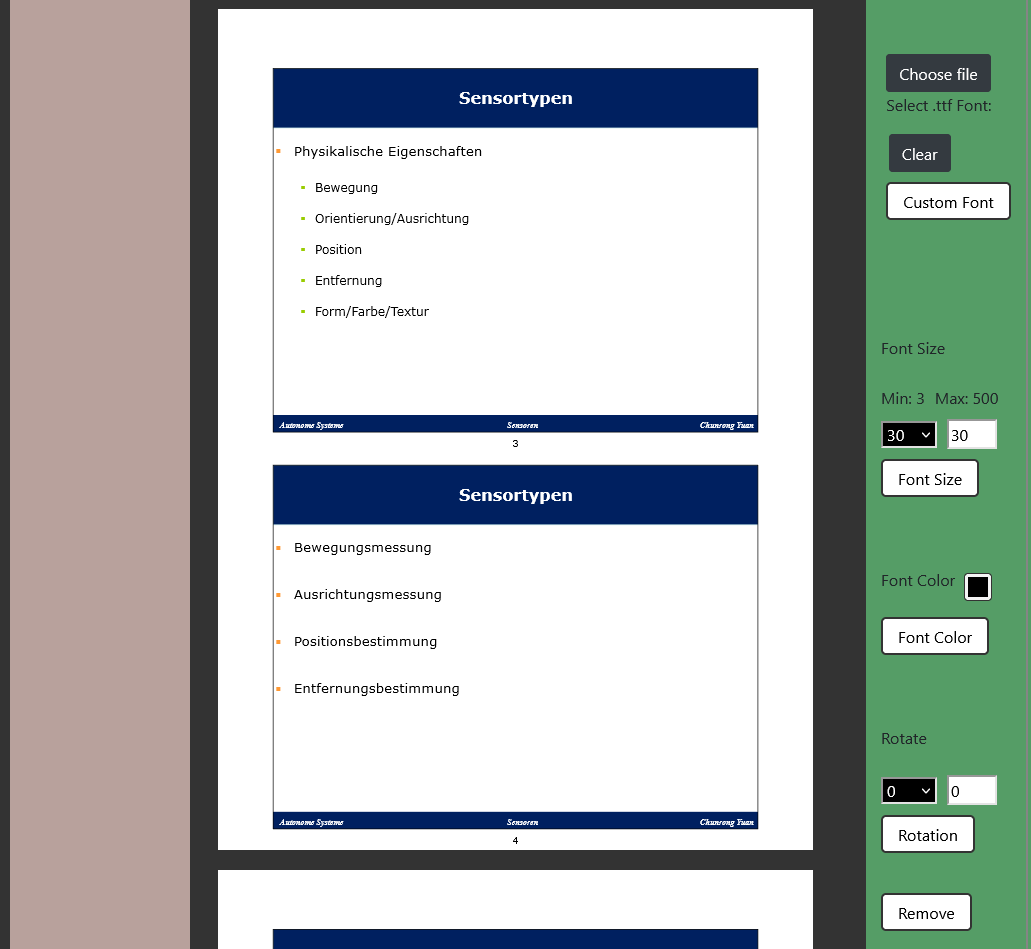
\includegraphics[width=1\textwidth]{"images/texteditor2.png"}
	\caption{Mehr Tools der Startseite des Writers der PDF Web App}
	\label{fig:texteditor2}
\end{figure}

Mit dem Button Text im Operations Bar und nachfolgendem Klick auf eine Seite, wird der Platzhaltertext dummy hinzugefügt. Unter dem Text erscheint eine dunkelrote controlBox, auf die alle Operationen des Operations Bars und in Tools im Box Mode angewendet werden können. Ich werde zunächst alle Operationen im Box Mode beschreiben und später auf den Layer Mode eingehen. Der Box Mode ist standardmäßig eingestellt. Operationen können durch die grünen Buttons zum Erstellen neuer Elemente, Delete und Move im Operations Bar und allen weißen Buttons in Tools getriggert werden. Wurde eine Operation ausgelöst, schaltet die Anwendung in den Modus dieser Operation. Darauffolgend können alle im Dokument verfügbaren controBoxes angeklickt werden, um die Operation auf das betreffende Element auszuführen. Alle Operationen in Tools beziehen sich jeweils auf das Element des aktuellen Editormoduls und sind nur auf diesem anwendbar. In der Praxis des Box Modes können mehrere Texte ohne erneute Betätigung des grünen Text-Buttons auf der Seite platziert werden. Für jedes neu hinzugefügte Editorelement wird eine Layer mit einem elementspezifischen Standardnamen und einem Index beginnend mit 1 in Layers erstellt. Die obere, linke Ecke der quadratischen controlBox sämtlicher Editorelemente wird an die Stelle positioniert, wo mit der Maus auf die Seite geklickt wurde. Alle controlBoxes werden nicht im Output-PDF gespeichert, denn sie dienen lediglich der Steuerung von Editorelementen, um Operationen im Box Mode anwenden zu können. Mit dem Delete-Button und nachfolgendem Klick in controlBoxes können Textelemente gelöscht werden. Move verschiebt einzelne Textelemente durch eine mit der Maus gedrückten und zur Zielposition bewegten controlBox. Sobald die Maus losgelassen wurde, wird der Text an der Zielposition aktualisiert. Dabei sollte eine controlBox langsam verschoben werden, denn der Mauszeiger muss sich innerhalb der controlBox bewegen. Delete und Move kommen in allen Editormodulen vor und funktionieren immer gleich. Ganz oben in Tools werden die x- und y-Koordinaten des Mauscursors auf der Seite angezeigt. Diese Mauscursorkoordinaten sind in jedem Editormodul präsent. 
\par
Textelemente lassen sich in der textarea editieren. Zeilenumbrüche werden berücksichtigt. Nachdem der dummy Text in der textarea überschrieben wurde, ein Klick auf den weißen Text-Button erfolgte und die Operation auf eine controlBox angewendet wurde, substituiert sich der Platzhaltertext mit dem aktuellen Text in der textarea. Die textarea kann in vertikaler Höhe expandiert werden. In allen Editormodulen werden jegliche Operationen in Tools exakt gleich ausgeführt: Einstellungen werden vorgenommen, der weiße Button für die jeweilige Operation wird betätigt und es wird auf eine oder mehrere controlBoxes geklickt. Unterhalb der Texteditierungsoperation kann der Zeilenabstand einstellt werden. Entweder kann das selection menu mit voreingestellten Werten betätigt werden oder ein benutzerdefinierter Wert im zugehörigen input field eingetippt werden. Neu hinzugefügte Elemente sind standardmäßig vorkonfiguriert. Alle selection menus und input fields sämtlicher Editormodule zeigen die Standardwerte der Konfiguration an. Bei jeder selection menu und input field-Kombination ist maßgeblich, welche Schaltfläche zuletzt betätigt wurde. Ein benutzerdefinierter Font als TTF- oder OTF-Datei lässt sich durch den dunkelgrauen Choose file-Button im Dateisystem auswählen. Er wird in einer Liste abgebildet und der zuletzt geöffnete Font wird ausgewählt. Die Auswahl des Fonts für die Custom Font-Operation wird durch einen Klick auf den radio button nebst Fontdateinamen aktiviert. Mittels Clear werden alle Fonts aus der Liste entfernt. Fontdateinamen werden nach 15 Zeichen in die nächste Zeile umgebrochen. Abbildung \ref{fig:custom-font} zeigt 2 geöffnete TTF-Schriftdateien in der Liste.

\begin{figure}[!htbp]
	\centering
	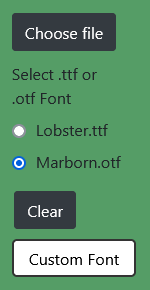
\includegraphics[width=0.2\textwidth]{"images/custom-font.png"}
	\caption{Benutzerdefinierte Fontliste im Texteditor der PDF Web App}
	\label{fig:custom-font}
\end{figure}

Die Fontgröße kann mittels selection menu und input field justiert werden. Bezüglich der Fontfarbe lässt sich ein Color Picker Menü mit Klick auf das initial schwarze Quadrat ausklappen. Es können Farbe und Transparenz eingestellt werden. Die Farbwerte stehen in den Formten RGBA, HSLA oder HEX zur Verfügung. Mit Klick auf die beiden kleinen senkrechten Pfeile im Color Picker wird das Format gewechselt. Das Menü des Color Pickers für die Fontfarbe ist in Abbildung \ref{fig:fontcolor} dargestellt. 

\begin{figure}[!htbp]
	\centering
	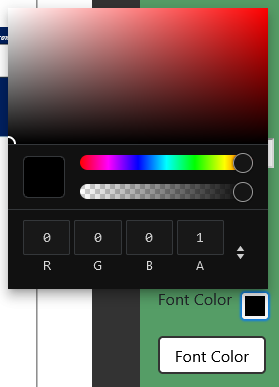
\includegraphics[width=0.5\textwidth]{"images/fontcolor.png"}
	\caption{Color picker für die Fontfarbe des Texteditors der PDF Web App}
	\label{fig:fontcolor}
\end{figure}

Als vorletzte Option kann der Text absolut gedreht werden. Durch den weißen Button Rotation und der entsprechenden Benutzerinteraktion durch selection Menu oder input field wird das Textelement rotiert. Absolute Rotation bedeutet, dass eine feste Rotationsskala angewendet wird, anhand der das Element rotiert wird. Bei einem Rotationswinkel von 0 Grad wird die Ausgangsrotation wiederhergestellt. Alle Editormodule arbeiten mit absoluter Rotation. Abschließend können alle Textelemente im Dokument mit dem Remove-Button gelöscht werden. Ein modifizierter Text wird in Abbildung \ref{fig:text} demonstriert.

\begin{figure}[!htbp]
	\centering
	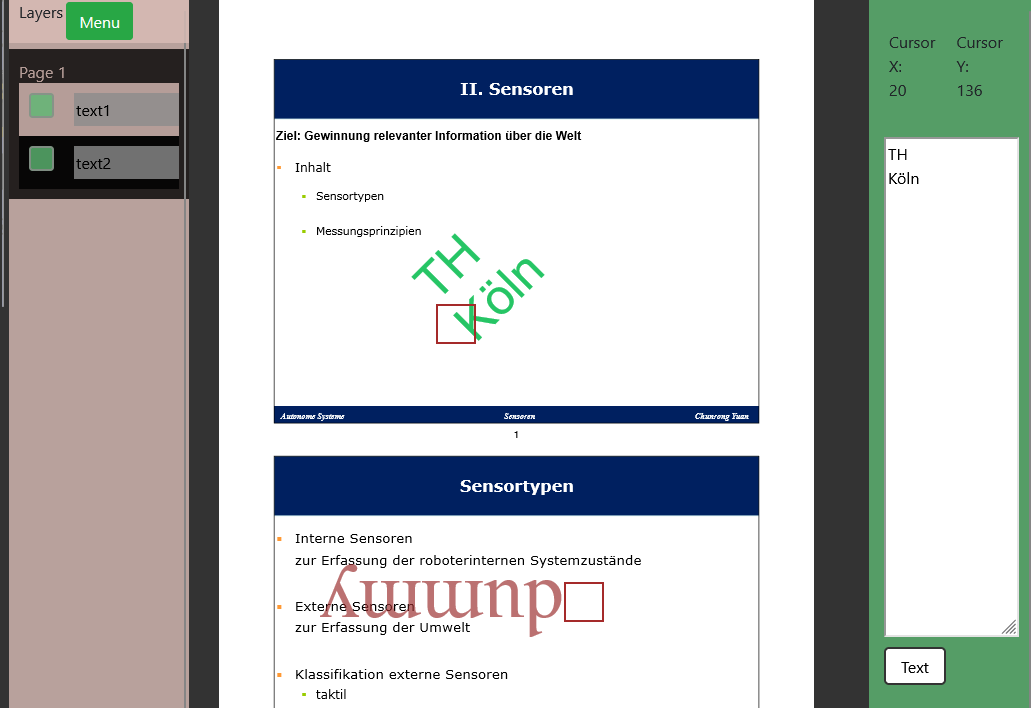
\includegraphics[width=1\textwidth]{"images/text.png"}
	\caption{Bearbeiteter Text im Writer der PDF Web App}
	\label{fig:text}
\end{figure}

\subsubsection{Drawings erstellen}
Der Drawer ist in Screenshot \ref{fig:drawer} abgebildet. 

\begin{figure}[!htbp]
	\centering
	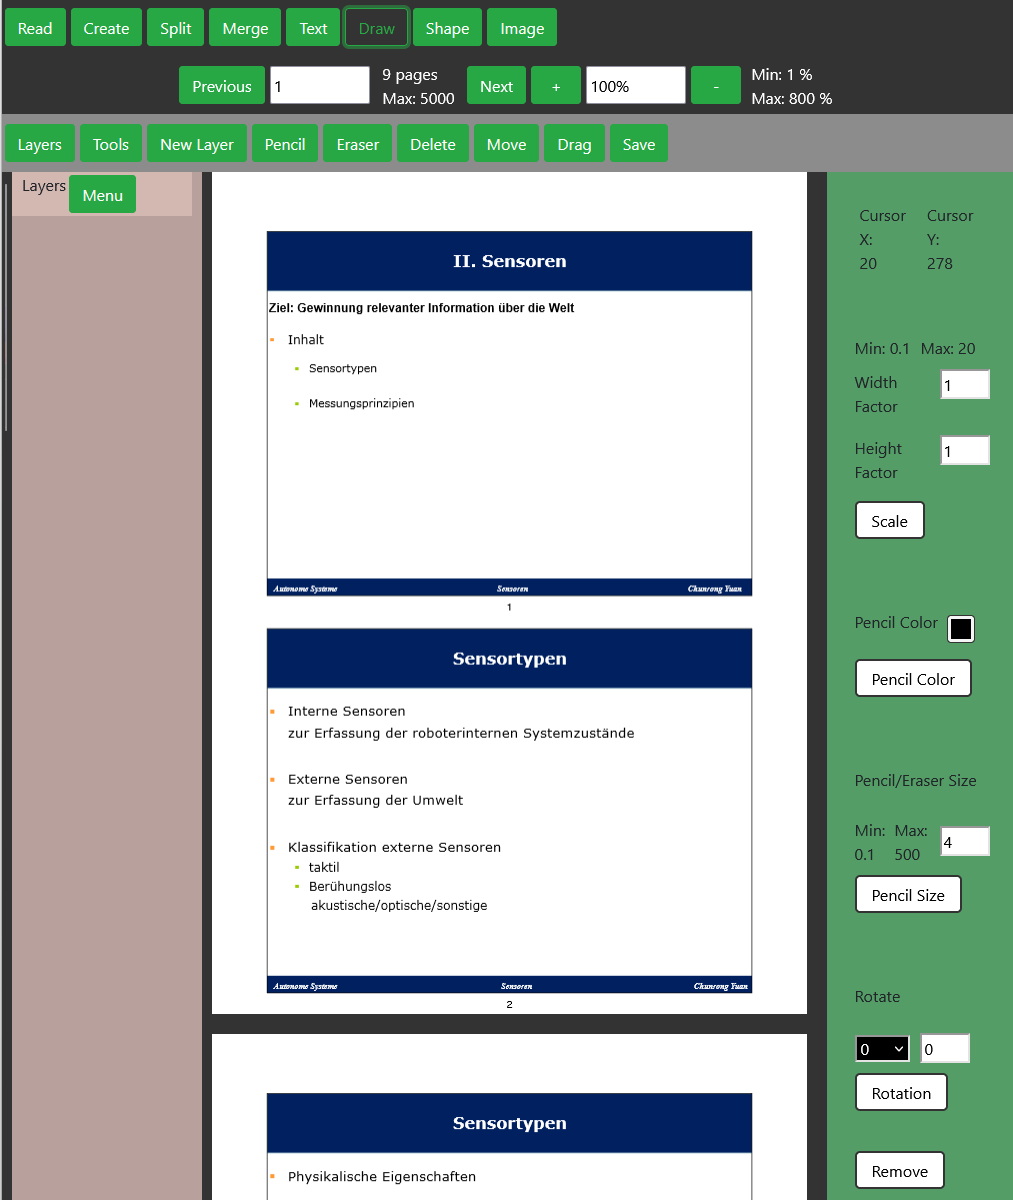
\includegraphics[width=1\textwidth]{"images/drawer.png"}
	\caption{Drawer der PDF Web App}
	\label{fig:drawer}
\end{figure}

Der Zeichenmodus wird mittels Pencil initiiert. Mit gedrückter Maustaste und gleichzeitigen Mausbewegungen erscheint eine Linie. Die Startstelle des Drawings wird durch eine magenta farbige controlBox markiert. Drawings lassen sich idealerweise mit einem Graphic Tablet erstellen. Für das erste Drawing der Seite wird von der Anwendung eine Layer zugewiesen. Mittels des New Layer-Buttons kann eine neue Layer kreiert werden. Falls keine Layer ausgewählt wurde, wird auf der zuletzt gezeichneten Layer der Seite gearbeitet. Generell wird auf der ausgewählten Layer gezeichnet. Der Radierermodus wird durch den Eraser-Button im Operations Bar aktiviert. Mit gedrückter Maustaste können Pixelbereiche des Drawings entfernt werden. Das Drawing zum Radieren wird durch die Auswahl der Layer bestimmt. Das Mauscursorsymbol der Zeichenoperation wird durch ein schwarzes, dünnes Kreuz signalisiert. Im Radierermodus alterniert das Mauscursorsymbol zu einem weißen, dicken Kreuz. Sobald eine Operation in Tools angewendet wird, wird der Zeichenmodus bzw. Radierermodus verlassen. In Tools kann ein Drawing relativ skaliert werden, indem ein Faktor eingegeben wird. Der Faktor kann auch ein Float sein und multipliziert sich immer mit der aktuellen Größe. Im nächsten Bereich definiert ein Color Picker die Stift- und Eraserfarbe inklusive der Deckkraft. Des Weiteren kann der Durchmesser des Stifts bzw. Radierers justiert werden. Ebenfalls können Drawings absolut rotiert werden. Wurde ein Drawing gedreht und auf der Layer weiter gezeichnet, so wird eine weitere Layer von der Anwendung angelegt. In der untersten Sektion von Tools entfernt Remove alle Drawings im Dokument. Teilweise transparente Drawings werden in Abbildung \ref{fig:drawing} dargestellt. 

\begin{figure}[!htbp]
	\centering
	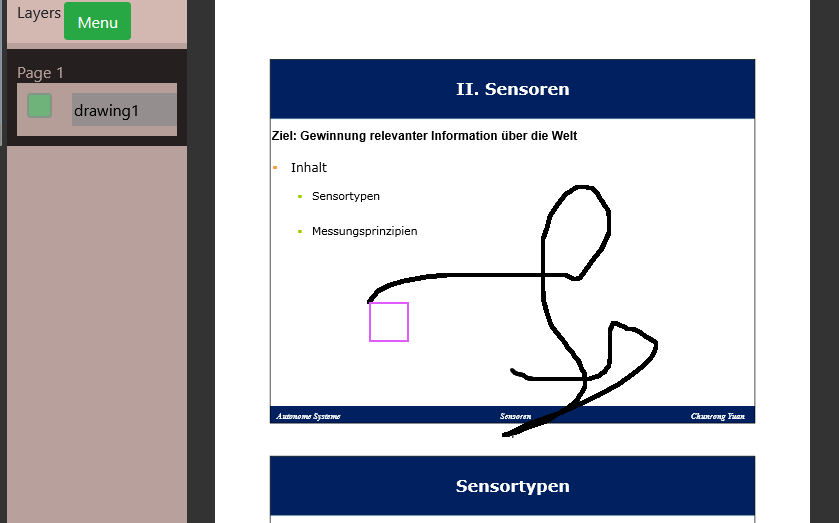
\includegraphics[width=1\textwidth]{"images/drawing.png"}
	\caption{Drawings im Drawer der PDF Web App}
	\label{fig:drawing}
\end{figure}


\subsubsection{Shapes hinzufügen}
Die Startseite des Shapers ist in den Screenshots \ref{fig:shaper} und \ref{fig:shaper2} abgebildet. 

\begin{figure}[!htbp]
	\centering
	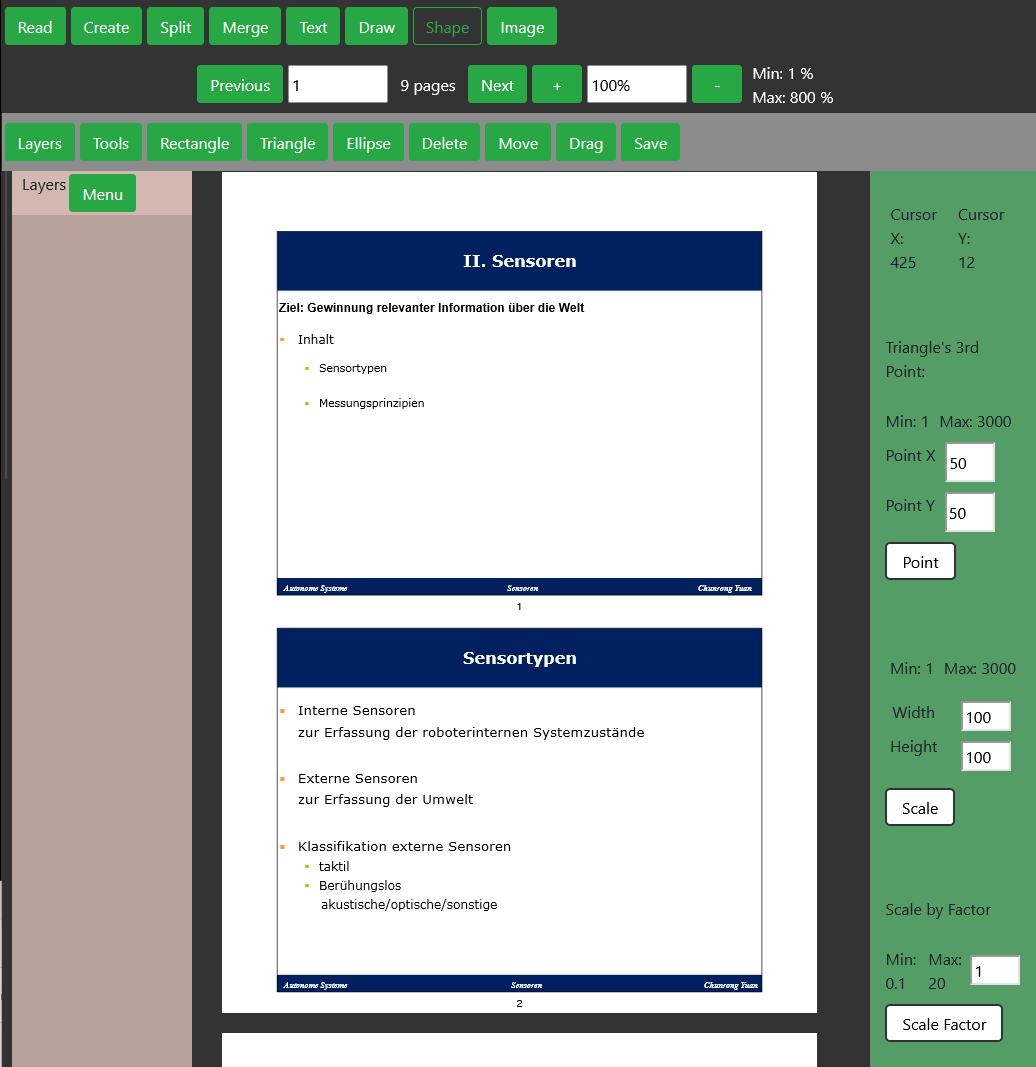
\includegraphics[width=1\textwidth]{"images/shaper.png"}
	\caption{Shaper der PDF Web App}
	\label{fig:shaper}
\end{figure}

\begin{figure}[!htbp]
	\centering
	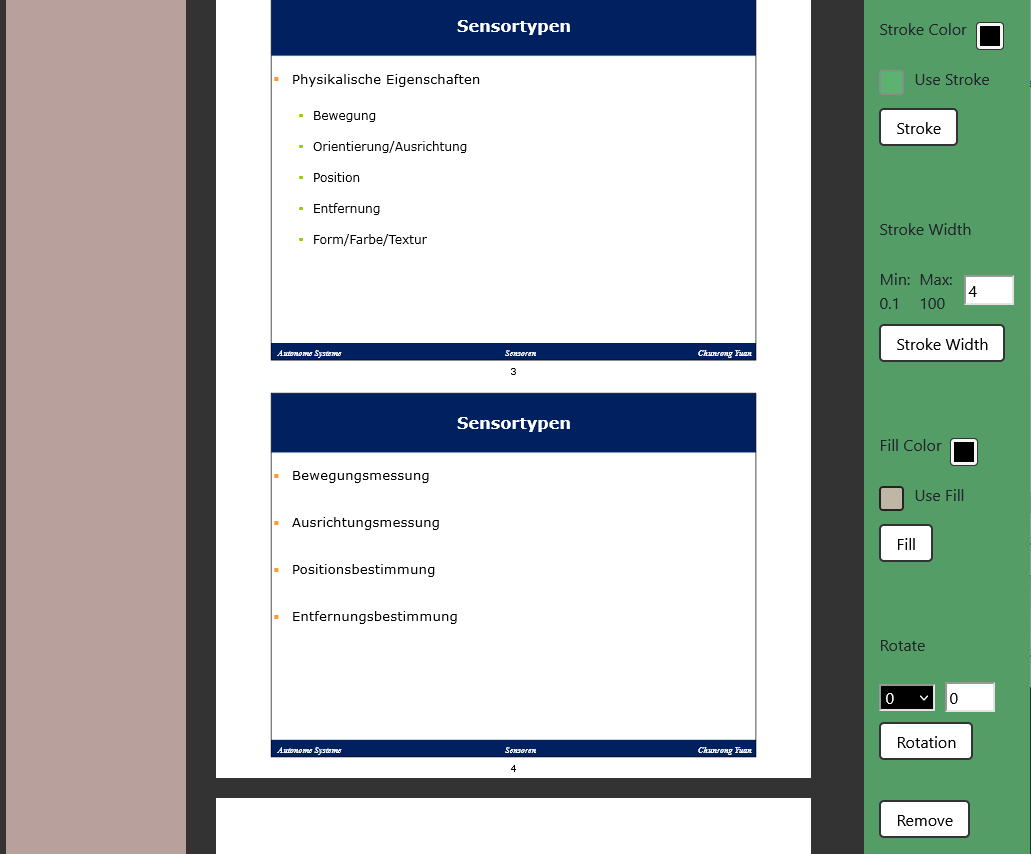
\includegraphics[width=1\textwidth]{"images/shaper2.png"}
	\caption{Mehr Tools des Shapers der PDF Web App}
	\label{fig:shaper2}
\end{figure}

Der Shapetyp kann durch die Buttons Rectangle für Rechteck, Triangle für Dreieck oder Ellipse und einem oder mehreren Klicks auf eine Seite bestimmt werden. Jedem Shape wird eine orange controlBox mehr oder weniger mittig hinzugefügt. In Tools des Shapers gibt es eine einzige Operation, die nur auf Dreiecke angewendet werden kann. Es handelt sich um die oberste Einstellung für die Breite und Höhe des dritten Punktes des Dreiecks (Triangle's Third Point). Mit dieser Operation kann der rechte Punkt der langen Spitze des default Dreiecks bearbeitet werden. Alle anderen Einstellmöglichkeiten können auf sämtlichen Shapeelementen Rectangle, Triangle und Ellipse arbeiten. Die Skalierung von Shapes bietet 2 Vorgehensweisen. Zum einen können Breite und Höhe unabhängig voneinander einstellt werden, was eine absolute Skalierung bedeutet. Zum anderen kann der proportionale, relative Skalierungsfaktor die Größe modulieren. Für die Umrandungslinien des Shapes kann auf der einen Seite die Farbe inklusive Deckkraft und auf der anderen Seite die Breite der Linie justiert werden. Die Strichfarbe muss mit der checkbox Use Stroke in Grün aktiviert sein. Bei Deaktivierung von Use Stroke schaltet sich automatisch die Use Fill checkbox ein und umgekehrt. Beide checkboxes können angehakt (Grün) sein, aber nicht beide zusammen abgehakt (Rosa). Use Fill muss Grün sein, um die Füllfarbe anzuwenden. Bei Strich- und Füllfarbe wird ein Color Picker verwendet. Alle Shapes können mit absoluter Rotation gedreht werden. Die controlBoxes werden durch die Rotation mitgedreht. Zuunterst entfernt der Remove-Button alle Shapes im Dokument. Der Screenshot \ref{fig:shaping} hebt mehrere bearbeitete Shapes hervor.

\begin{figure}[!htbp]
	\centering
	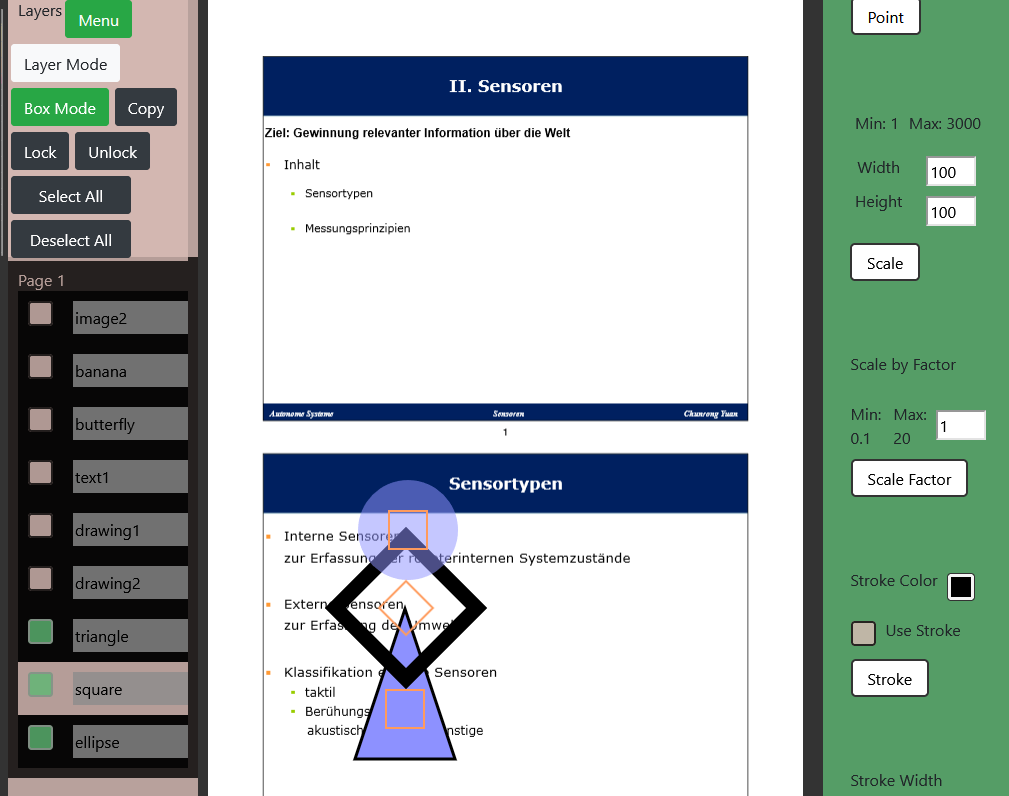
\includegraphics[width=1\textwidth]{"images/shaping.png"}
	\caption{Shapes im Shaper der PDF Web App}
	\label{fig:shaping}
\end{figure}


\subsubsection{Images einfügen}
Der Imager ist in Bild \ref{fig:images} dargestellt. 

\begin{figure}[!htbp]
	\centering
	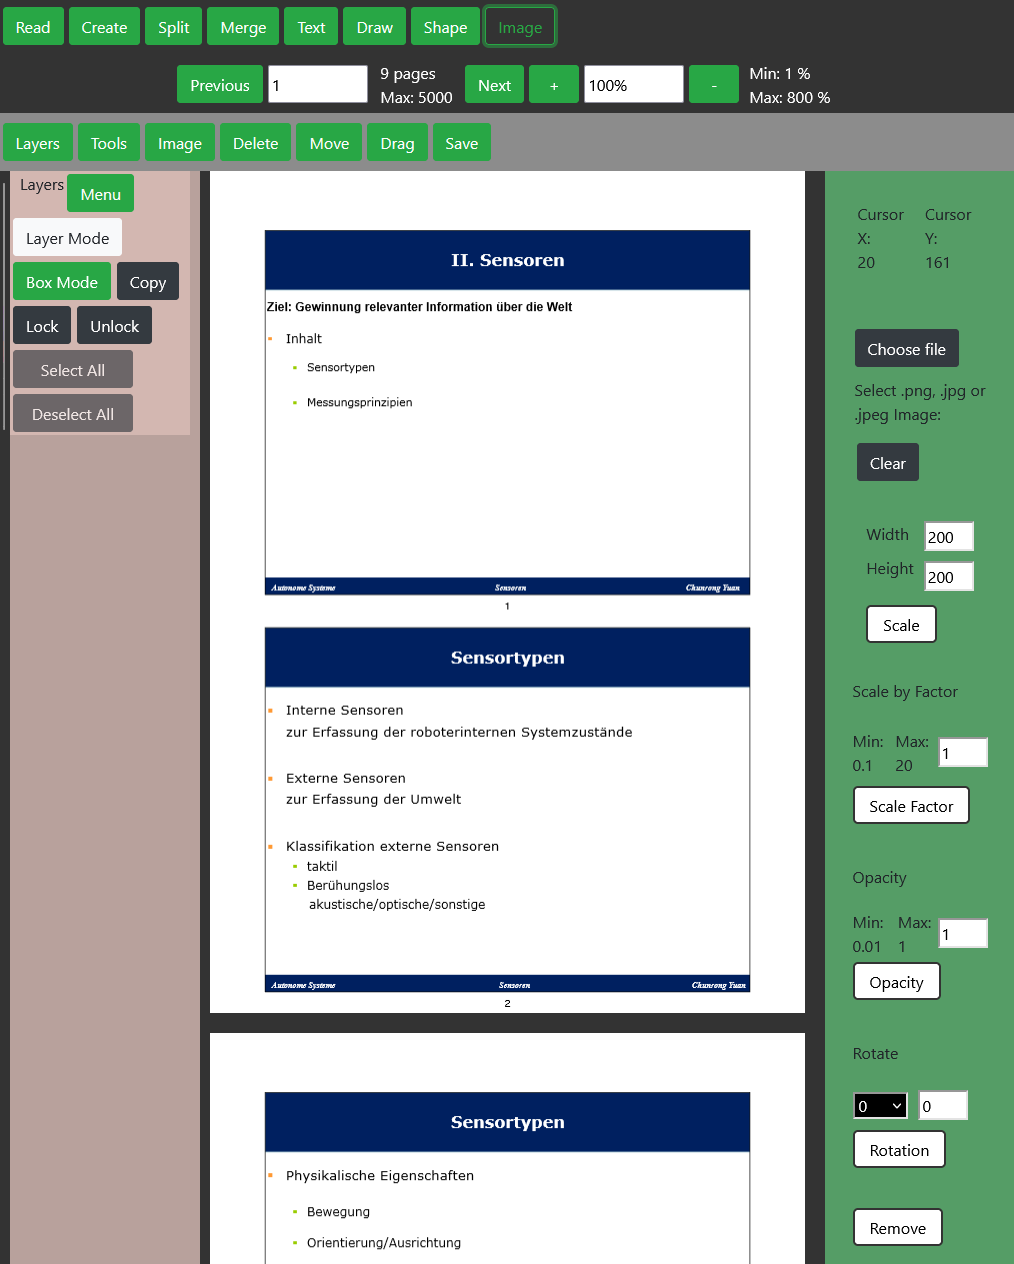
\includegraphics[width=1\textwidth]{"images/images.png"}
	\caption{Imager der PDF Web App}
	\label{fig:images}
\end{figure}

Um ein Image mit dem Image-Button im Operations Bar hinzuzufügen, muss zunächst ein Image mittels des dunkelgrauen Choose file-Buttons im Dateisystem ausgewählt werden. Dadurch erscheint der Imagename in der Liste unter Choose file. Mehrere Images lassen sich nacheinander mittels des Dateidialogs auswählen. Das zuletzt selektierte Image wird automatisch mit einem blauen radio button gekennzeichnet. Zusätzlich werden die Originaldimensionen des Images angezeigt, sobald das Image mittels des grünen Buttons Image im Operations Bar auf der Seite platziert wurde. Eine hellblaue controlBox erscheint bei der Imageplatzierung. Ein Image kann in Breite und Höhe absolut skaliert werden. Auf proportionale Art und Weise wird ein Image mit dem relativen Skalierungsfaktor verkleinert bzw. vergrößert. Unterhalb der Skalierungsoperationen kann die Deckkraft eines Images bestimmt werden. Ebenfalls lässt sich ein Image absolut rotieren. Zuletzt können alle Images im Dokument mit dem Remove-Button entfernt werden. Die Abbildung \ref{fig:imaging} zeigt den Imager in Aktion.

\begin{figure}[!htbp]
	\centering
	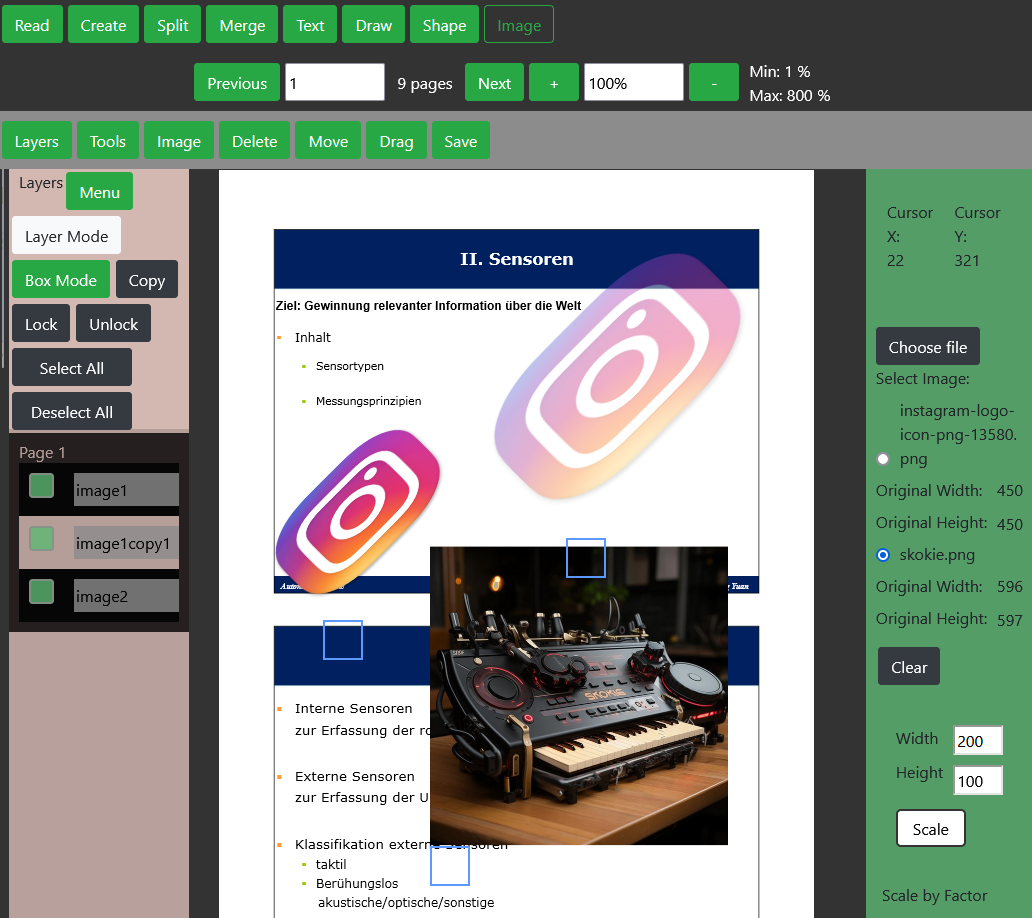
\includegraphics[width=1\textwidth]{"images/imaging.png"}
	\caption{Platzierte Images im Imager der PDF Web App}
	\label{fig:imaging}
\end{figure}

\subsubsection{Ebenensteuerung}
Das in Abbildung \ref{fig:ebenenmenu} gezeigte Layers Menu lässt sich mit einem Klick auf Menu in Layers hervorholen oder verbergen. Es ist möglich durch die Liste an hinzugefügten Layers zu scrollen.

\begin{figure}[!htbp]
	\centering
	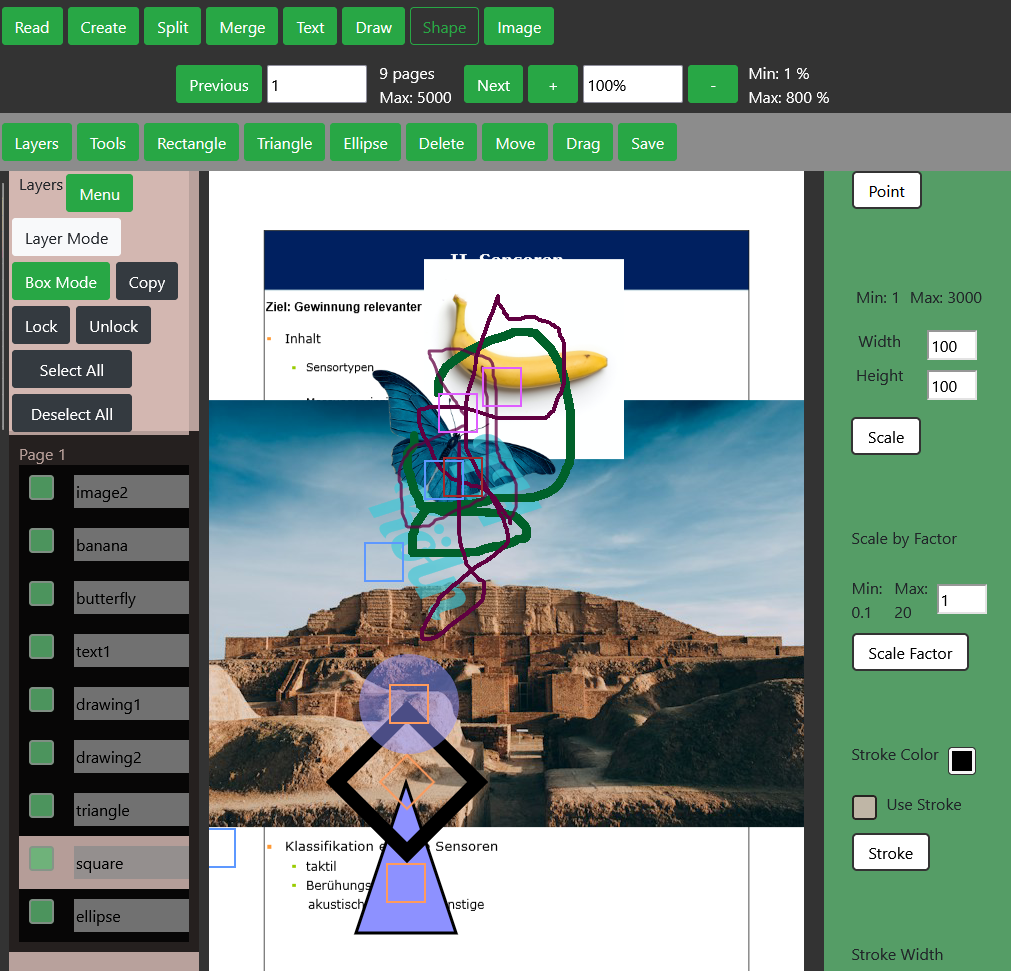
\includegraphics[width=1\textwidth]{"images/ebenenmenu.png"}
	\caption{Ausgeklapptes Layers Menu im Editor der PDF Web App}
	\label{fig:ebenenmenu}
\end{figure}

Standardmäßig sind die Schaltflächen eingeklappt. Jedem hinzugefügtem Element wird eine automatisch ausgewählte Layer zugewiesen. Gruppiert werden sie nach aufsteigenden Seitenzahlen. Mit Platzierung eines Elements auf einer neuen Seite bildet sich die Seitengruppe. Die Farbe Rosa kennzeichnet eine ausgewählte Layer und die Farbe Schwarz eine abgewählte. Mehrere Layers können zeitgleich ausgewählt sein. Eine neu angelegte Layer wird standardmäßig benannt. Der Standardname setzt sich aus dem Elementtyp und einem nummerischen Index, beginnend mit 1, zusammen. Dieser lässt sich im grauen input field auf der Layer überschreiben. Im Layers Menu ist ein Wechsel zwischen Box Mode und Layer Mode möglich. Ein grüner Modus-Button signalisiert einen aktiven Modus, wohingegen ein weißer Button eine Inaktivität symbolisiert. Der Box Mode oder Layer Mode sind nur exklusiv aktiv. Mittels des dunkelgrauen Copy-Buttons lassen sich ausgewählte Layers samt ihrer Elemente duplizieren. Die Copy-Operation schlägt sich im Layernamen nieder: Layername + copy + Index beginnend mit 1. Layers können durch Lock und Unlock gesperrt bzw. entsperrt werden (Schreibschutz ihrer Elemente). Eine locked, unausgewählte Layer wird in Weiß und eine locked, ausgewählte ist Rosa mit weißer Umrandung signalisiert. 

\begin{figure}[!htbp]
	\centering
	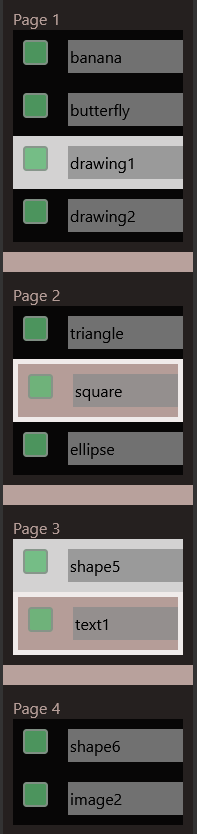
\includegraphics[width=0.3\textwidth]{"images/ebenen.png"}
	\caption{Teilweise locked Layers im Editor der PDF Web App}
	\label{fig:ebenen}
\end{figure}

Die dunkelgrauen Select All und Deselect All Buttons stellen Auswahlfilter dar. Sobald die Maus auf die Buttons bewegt wird, klappt sich ein Selection Filter Menu auf. Über Select All lassen sich mehrere Layers basierend auf Seitenzahlen, dem Elementtyp und locked/unlocked selektieren. Aktivierte Selection Filter-Buttons färben sich grün und deaktivierte weiß. In der Seitenliste müssen Seitenzahlen durch Kommas abgetrennt werden. Die Filter werden mittels Select All angewendet. Im Falle einer leeren Seitenliste und inaktiven Buttons werden alle Layers dokumentübergreifend ausgewählt. Deselect All funktioniert analog bezogen auf Auswahl aufheben. Der Bildausschnitt \ref{fig:filtering} enthält ein Beispiel von Deselect All. Gemäß des Beispiels wird die Auswahl auf allen unlocked Textelementen auf Seite 1 und 2 aufgehoben. 

\begin{figure}[!htbp]
	\centering
	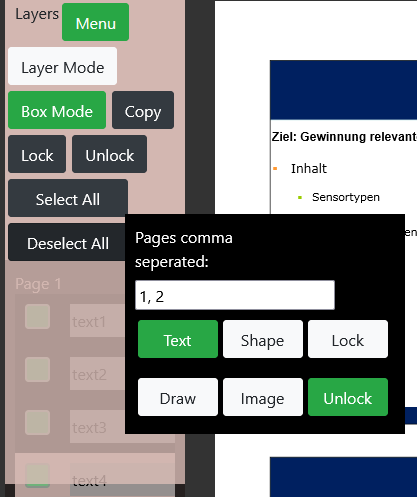
\includegraphics[width=0.6\textwidth]{"images/filtering.png"}
	\caption{Deselection Filter Menu mit aktivierten Filtern im Editor der PDF Web App}
	\label{fig:filtering}
\end{figure}

Sowohl bei Select All als auch Deselect All greift die Input Control im input field der Seitenliste. Sofern ungültige Eingaben vorliegen, z.B. Seiten sind als Floats oder Strings deklariert, wird die Eingabe gelöscht – bei Auslösung des Filters. Die Reihenfolge der Elemente im Vorder- bzw. Hintergrund kann über die Layerreihenfolge gesteuert werden. Untere Layers auf dem Stapel einer Seitengruppe liegen im Vordergrund der Seite. Einzelne Layers können auf eine Ziellayer mit gedrückter Maustaste verschoben werden. Dabei ändert sich das Maussymbol. Die Verschiebung funktioniert seitenübergreifend. Linksseitig des Layernamens steuert eine grüne checkbox die Sichtbarkeit der Layer und ihres Elements. Eine grüne checkbox resultiert in Sichtbarkeit und eine rosa in Unsichtbarkeit. Ausgeblendete oder locked Layers können kopiert und in den Vordergrund bzw. Hintergrund oder auf eine andere Seite verschoben werden. Ebenso können ausgeblendete Layers gesperrt und locked Layers ausgeblendet werden. Operationen im Layer Mode können auf ausgeblendete Layers angewendet werden.

\subsubsection{Arbeiten im Layer Mode}
Ich habe bisher alle Operationen im Box Mode beschrieben. Es gibt außerdem den Layer Mode. Im Layer Mode können mehrere Layers selektiert werden. Die Operationen Move, Delete und alle Operationen in Tools können auf alle selektierten Layers angewendet werden. In der Umsetzung wird der Button der gewünschten Operation angesteuert und diese wird auf den Layers ausgeführt. In diesem Vorgang sind die Operationen in Tools elementspezifisch. Wird beispielsweise eine Tools-Einstellung des Writers auf Text und Shape Layers angewendet, wird die Operation lediglich auf Text ausgeführt. Delete und Move operieren in jedem Editormodul im Layer Mode auf allen Elementtypen. Während der Move-Operation wird die controlBox mit gedrückter Maustaste an die Zielposition verschoben. Alle weiteren Layers, die zusätzlich ausgewählt wurden, werden mit gleichem proportionalem Abstand zueinander um die gewünschten Verschiebungskoordinaten verschoben. 